\documentclass[tikz,crop,convert={density=200,outext=.png},border=0.4cm]{standalone}

\usepackage{pgfplots}
\usepackage{amsmath}
\usetikzlibrary{arrows.meta}
\usepackage{physics}
\usepackage{xcolor}
\definecolor{mixed_1}{RGB}{8,48,107}
\definecolor{pow_1}{RGB}{103,0,31}
\pgfplotsset{compat=newest,
    %width=6cm,
    %height=3cm,
    scale only axis=true,
    max space between ticks=25pt,
    try min ticks=5,
    every axis/.style={
        axis y line=middle,
        axis x line=middle,
        axis line style={thick,->,>=latex, shorten >=-.3cm}
    },
    every axis plot/.append style={thick},
    tick style={black, thick},
}
\tikzset{
    semithick/.style={line width=0.8pt},
}
\usepgfplotslibrary{groupplots}
\usepgfplotslibrary{dateplot}
% Document begins
\begin{document}
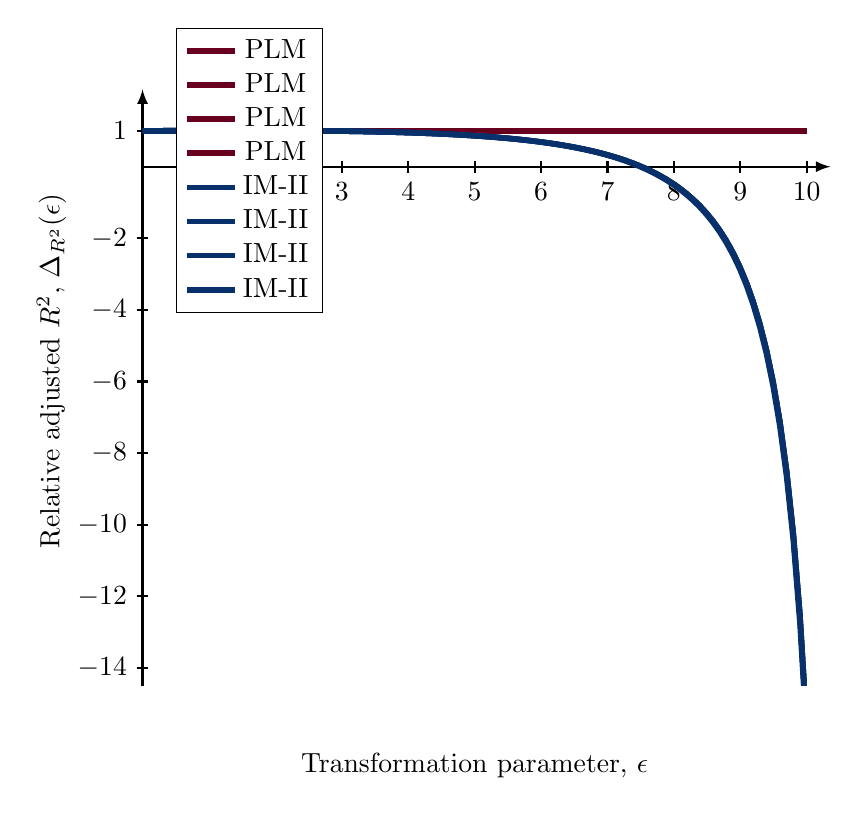
\begin{tikzpicture}
  % The axis of the plot
\begin{axis}[
    %title={Model: $\dv{y}{t}=\frac{2y}{t}$ with solution $y(t)=C_1t^2$\\Symmetry: $\Gamma_{\epsilon}=(t,y)\mapsto\left(\exp\left(\epsilon\right)t,\exp\left(-\epsilon\right)y\right)$},
    title style = {align=left},
    xlabel={Transformation parameter, $\epsilon$},
    ylabel={Relative adjusted $R^2$, $\Delta_{R^2}(\epsilon)$},
    %ylabel={Logarithm of Incidence, $\ln\left(R(t)\right)$},    
    % ylabel={Incidence, $R(t)$},
    x label style={at={(axis description cs:0.5,-0.1)},anchor=north},
    y label style={at={(axis description cs:-0.1,0.55)},rotate=90,anchor=south},    
    % xmin=-27, xmax=5,
    %xmin=0, xmax=10,
    %xtick={0,12,20,...,60,70,82},    
    ymin=-14.5, ymax=1.5,
    %xtick={-30,-27,...,9},
    ytick={1,0,-2,-4,-6,-8,-10,-12,-14},
    legend style={at={(axis description cs:0.05,0.9)},anchor=west},    
    %legend pos=north west,
    %ymajorgrids=true,
    grid style=dashed,
]
% Plot the data
\addplot[
color=pow_1,line width=2pt,
]
coordinates {%
(0.0,1.0)
(0.10101010101010101,1.000000000000051)
(0.20202020202020202,0.999999999998303)
(0.30303030303030304,1.0000000000001539)
(0.40404040404040403,0.9999999999983028)
(0.5050505050505051,1.0000000000002565)
(0.6060606060606061,1.000000000000307)
(0.7070707070707071,0.999999999998303)
(0.8080808080808081,1.0000000000004097)
(0.9090909090909091,1.0000000000004612)
(1.0101010101010102,0.9999999999983027)
(1.1111111111111112,1.0000000000005638)
(1.2121212121212122,0.9999999999983029)
(1.3131313131313131,0.9999999999983028)
(1.4141414141414141,0.9999999999983028)
(1.5151515151515151,1.0000000000007685)
(1.6161616161616161,0.9999999999983029)
(1.7171717171717171,1.000000000000871)
(1.8181818181818181,0.9999999999983028)
(1.9191919191919191,1.0000000000009743)
(2.0202020202020203,1.0000000000010254)
(2.121212121212121,1.0000000000010765)
(2.2222222222222223,1.000000000001128)
(2.323232323232323,1.0000000000011795)
(2.4242424242424243,0.9999999999983029)
(2.525252525252525,0.9999999999983028)
(2.6262626262626263,1.0000000000013323)
(2.727272727272727,0.9999999999983029)
(2.8282828282828283,0.9999999999983028)
(2.929292929292929,0.9999999999983029)
(3.0303030303030303,0.9999999999983029)
(3.131313131313131,1.0000000000015896)
(3.2323232323232323,0.9999999999983029)
(3.3333333333333335,0.9999999999983028)
(3.4343434343434343,0.999999999998303)
(3.5353535353535355,1.0000000000017943)
(3.6363636363636362,1.0000000000018454)
(3.7373737373737375,1.0000000000018974)
(3.8383838383838382,1.0000000000019478)
(3.9393939393939394,1.0000000000019993)
(4.040404040404041,1.0000000000020506)
(4.141414141414141,0.9999999999983028)
(4.242424242424242,0.9999999999983029)
(4.343434343434343,0.9999999999983028)
(4.444444444444445,1.0000000000022569)
(4.545454545454545,1.0000000000023075)
(4.646464646464646,0.9999999999983028)
(4.747474747474747,0.9999999999983029)
(4.848484848484849,1.0000000000024623)
(4.94949494949495,1.000000000002512)
(5.05050505050505,0.999999999998303)
(5.151515151515151,1.0000000000026144)
(5.252525252525253,1.0000000000026665)
(5.353535353535354,1.000000000002718)
(5.454545454545454,0.9999999999983027)
(5.555555555555555,1.0000000000028204)
(5.656565656565657,1.0000000000028708)
(5.757575757575758,1.0000000000029228)
(5.858585858585858,0.9999999999983029)
(5.959595959595959,0.9999999999983027)
(6.0606060606060606,1.0000000000030764)
(6.161616161616162,1.0000000000031275)
(6.262626262626262,1.0000000000031783)
(6.363636363636363,1.0000000000032296)
(6.4646464646464645,1.000000000003282)
(6.565656565656566,1.0000000000033318)
(6.666666666666667,1.000000000003384)
(6.767676767676767,1.0000000000034348)
(6.8686868686868685,1.0000000000034859)
(6.96969696969697,0.9999999999983027)
(7.070707070707071,1.00000000000359)
(7.171717171717171,1.000000000003641)
(7.2727272727272725,1.0000000000036908)
(7.373737373737374,0.999999999998303)
(7.474747474747475,1.000000000003795)
(7.575757575757575,0.9999999999983027)
(7.6767676767676765,1.0000000000038956)
(7.777777777777778,0.9999999999983027)
(7.878787878787879,0.9999999999983029)
(7.979797979797979,1.0000000000040505)
(8.080808080808081,1.0000000000041016)
(8.181818181818182,1.0000000000041547)
(8.282828282828282,0.9999999999983031)
(8.383838383838384,0.9999999999983029)
(8.484848484848484,1.0000000000043072)
(8.585858585858587,1.0000000000043585)
(8.686868686868687,0.999999999998303)
(8.787878787878787,1.0000000000044604)
(8.88888888888889,0.9999999999983029)
(8.98989898989899,1.0000000000045648)
(9.09090909090909,1.000000000004614)
(9.191919191919192,1.0000000000046658)
(9.292929292929292,1.000000000004718)
(9.393939393939394,1.000000000004769)
(9.494949494949495,0.9999999999983032)
(9.595959595959595,1.0000000000048725)
(9.696969696969697,1.0000000000049225)
(9.797979797979798,1.0000000000049725)
(9.8989898989899,1.0000000000050229)
(10.0,1.0000000000050784)
};
\addlegendentry{PLM}
\addplot[
color=pow_1,line width=2pt,
]
coordinates {%
(0.0,1.0)
(0.10101010101010101,1.000000000000051)
(0.20202020202020202,0.999999999998303)
(0.30303030303030304,1.0000000000001539)
(0.40404040404040403,0.9999999999983028)
(0.5050505050505051,1.0000000000002565)
(0.6060606060606061,1.000000000000307)
(0.7070707070707071,0.999999999998303)
(0.8080808080808081,1.0000000000004097)
(0.9090909090909091,1.0000000000004612)
(1.0101010101010102,0.9999999999983027)
(1.1111111111111112,1.0000000000005638)
(1.2121212121212122,0.9999999999983029)
(1.3131313131313131,0.9999999999983028)
(1.4141414141414141,0.9999999999983028)
(1.5151515151515151,1.0000000000007685)
(1.6161616161616161,0.9999999999983029)
(1.7171717171717171,1.000000000000871)
(1.8181818181818181,0.9999999999983028)
(1.9191919191919191,1.0000000000009743)
(2.0202020202020203,1.0000000000010254)
(2.121212121212121,1.0000000000010765)
(2.2222222222222223,1.000000000001128)
(2.323232323232323,1.0000000000011795)
(2.4242424242424243,0.9999999999983029)
(2.525252525252525,0.9999999999983028)
(2.6262626262626263,1.0000000000013323)
(2.727272727272727,0.9999999999983029)
(2.8282828282828283,0.9999999999983028)
(2.929292929292929,0.9999999999983029)
(3.0303030303030303,0.9999999999983029)
(3.131313131313131,1.0000000000015896)
(3.2323232323232323,0.9999999999983029)
(3.3333333333333335,0.9999999999983028)
(3.4343434343434343,0.999999999998303)
(3.5353535353535355,1.0000000000017943)
(3.6363636363636362,1.0000000000018454)
(3.7373737373737375,1.0000000000018974)
(3.8383838383838382,1.0000000000019478)
(3.9393939393939394,1.0000000000019993)
(4.040404040404041,1.0000000000020506)
(4.141414141414141,0.9999999999983028)
(4.242424242424242,0.9999999999983029)
(4.343434343434343,0.9999999999983028)
(4.444444444444445,1.0000000000022569)
(4.545454545454545,1.0000000000023075)
(4.646464646464646,0.9999999999983028)
(4.747474747474747,0.9999999999983029)
(4.848484848484849,1.0000000000024623)
(4.94949494949495,1.000000000002512)
(5.05050505050505,0.999999999998303)
(5.151515151515151,1.0000000000026144)
(5.252525252525253,1.0000000000026665)
(5.353535353535354,1.000000000002718)
(5.454545454545454,0.9999999999983027)
(5.555555555555555,1.0000000000028204)
(5.656565656565657,1.0000000000028708)
(5.757575757575758,1.0000000000029228)
(5.858585858585858,0.9999999999983029)
(5.959595959595959,0.9999999999983027)
(6.0606060606060606,1.0000000000030764)
(6.161616161616162,1.0000000000031275)
(6.262626262626262,1.0000000000031783)
(6.363636363636363,1.0000000000032296)
(6.4646464646464645,1.000000000003282)
(6.565656565656566,1.0000000000033318)
(6.666666666666667,1.000000000003384)
(6.767676767676767,1.0000000000034348)
(6.8686868686868685,1.0000000000034859)
(6.96969696969697,0.9999999999983027)
(7.070707070707071,1.00000000000359)
(7.171717171717171,1.000000000003641)
(7.2727272727272725,1.0000000000036908)
(7.373737373737374,0.999999999998303)
(7.474747474747475,1.000000000003795)
(7.575757575757575,0.9999999999983027)
(7.6767676767676765,1.0000000000038956)
(7.777777777777778,0.9999999999983027)
(7.878787878787879,0.9999999999983029)
(7.979797979797979,1.0000000000040505)
(8.080808080808081,1.0000000000041016)
(8.181818181818182,1.0000000000041547)
(8.282828282828282,0.9999999999983031)
(8.383838383838384,0.9999999999983029)
(8.484848484848484,1.0000000000043072)
(8.585858585858587,1.0000000000043585)
(8.686868686868687,0.999999999998303)
(8.787878787878787,1.0000000000044604)
(8.88888888888889,0.9999999999983029)
(8.98989898989899,1.0000000000045648)
(9.09090909090909,1.000000000004614)
(9.191919191919192,1.0000000000046658)
(9.292929292929292,1.000000000004718)
(9.393939393939394,1.000000000004769)
(9.494949494949495,0.9999999999983032)
(9.595959595959595,1.0000000000048725)
(9.696969696969697,1.0000000000049225)
(9.797979797979798,1.0000000000049725)
(9.8989898989899,1.0000000000050229)
(10.0,1.0000000000050784)
};
\addlegendentry{PLM}
\addplot[
color=pow_1,line width=2pt,
]
coordinates {%
(0.0,1.0)
(0.10101010101010101,1.000000000000051)
(0.20202020202020202,0.999999999998303)
(0.30303030303030304,1.0000000000001539)
(0.40404040404040403,0.9999999999983028)
(0.5050505050505051,1.0000000000002565)
(0.6060606060606061,1.000000000000307)
(0.7070707070707071,0.999999999998303)
(0.8080808080808081,1.0000000000004097)
(0.9090909090909091,1.0000000000004612)
(1.0101010101010102,0.9999999999983027)
(1.1111111111111112,1.0000000000005638)
(1.2121212121212122,0.9999999999983029)
(1.3131313131313131,0.9999999999983028)
(1.4141414141414141,0.9999999999983028)
(1.5151515151515151,1.0000000000007685)
(1.6161616161616161,0.9999999999983029)
(1.7171717171717171,1.000000000000871)
(1.8181818181818181,0.9999999999983028)
(1.9191919191919191,1.0000000000009743)
(2.0202020202020203,1.0000000000010254)
(2.121212121212121,1.0000000000010765)
(2.2222222222222223,1.000000000001128)
(2.323232323232323,1.0000000000011795)
(2.4242424242424243,0.9999999999983029)
(2.525252525252525,0.9999999999983028)
(2.6262626262626263,1.0000000000013323)
(2.727272727272727,0.9999999999983029)
(2.8282828282828283,0.9999999999983028)
(2.929292929292929,0.9999999999983029)
(3.0303030303030303,0.9999999999983029)
(3.131313131313131,1.0000000000015896)
(3.2323232323232323,0.9999999999983029)
(3.3333333333333335,0.9999999999983028)
(3.4343434343434343,0.999999999998303)
(3.5353535353535355,1.0000000000017943)
(3.6363636363636362,1.0000000000018454)
(3.7373737373737375,1.0000000000018974)
(3.8383838383838382,1.0000000000019478)
(3.9393939393939394,1.0000000000019993)
(4.040404040404041,1.0000000000020506)
(4.141414141414141,0.9999999999983028)
(4.242424242424242,0.9999999999983029)
(4.343434343434343,0.9999999999983028)
(4.444444444444445,1.0000000000022569)
(4.545454545454545,1.0000000000023075)
(4.646464646464646,0.9999999999983028)
(4.747474747474747,0.9999999999983029)
(4.848484848484849,1.0000000000024623)
(4.94949494949495,1.000000000002512)
(5.05050505050505,0.999999999998303)
(5.151515151515151,1.0000000000026144)
(5.252525252525253,1.0000000000026665)
(5.353535353535354,1.000000000002718)
(5.454545454545454,0.9999999999983027)
(5.555555555555555,1.0000000000028204)
(5.656565656565657,1.0000000000028708)
(5.757575757575758,1.0000000000029228)
(5.858585858585858,0.9999999999983029)
(5.959595959595959,0.9999999999983027)
(6.0606060606060606,1.0000000000030764)
(6.161616161616162,1.0000000000031275)
(6.262626262626262,1.0000000000031783)
(6.363636363636363,1.0000000000032296)
(6.4646464646464645,1.000000000003282)
(6.565656565656566,1.0000000000033318)
(6.666666666666667,1.000000000003384)
(6.767676767676767,1.0000000000034348)
(6.8686868686868685,1.0000000000034859)
(6.96969696969697,0.9999999999983027)
(7.070707070707071,1.00000000000359)
(7.171717171717171,1.000000000003641)
(7.2727272727272725,1.0000000000036908)
(7.373737373737374,0.999999999998303)
(7.474747474747475,1.000000000003795)
(7.575757575757575,0.9999999999983027)
(7.6767676767676765,1.0000000000038956)
(7.777777777777778,0.9999999999983027)
(7.878787878787879,0.9999999999983029)
(7.979797979797979,1.0000000000040505)
(8.080808080808081,1.0000000000041016)
(8.181818181818182,1.0000000000041547)
(8.282828282828282,0.9999999999983031)
(8.383838383838384,0.9999999999983029)
(8.484848484848484,1.0000000000043072)
(8.585858585858587,1.0000000000043585)
(8.686868686868687,0.999999999998303)
(8.787878787878787,1.0000000000044604)
(8.88888888888889,0.9999999999983029)
(8.98989898989899,1.0000000000045648)
(9.09090909090909,1.000000000004614)
(9.191919191919192,1.0000000000046658)
(9.292929292929292,1.000000000004718)
(9.393939393939394,1.000000000004769)
(9.494949494949495,0.9999999999983032)
(9.595959595959595,1.0000000000048725)
(9.696969696969697,1.0000000000049225)
(9.797979797979798,1.0000000000049725)
(9.8989898989899,1.0000000000050229)
(10.0,1.0000000000050784)
};
\addlegendentry{PLM}
\addplot[
color=pow_1,line width=2pt,
]
coordinates {%
(0.0,1.0)
(0.10101010101010101,1.000000000000051)
(0.20202020202020202,0.999999999998303)
(0.30303030303030304,1.0000000000001539)
(0.40404040404040403,0.9999999999983028)
(0.5050505050505051,1.0000000000002565)
(0.6060606060606061,1.000000000000307)
(0.7070707070707071,0.999999999998303)
(0.8080808080808081,1.0000000000004097)
(0.9090909090909091,1.0000000000004612)
(1.0101010101010102,0.9999999999983027)
(1.1111111111111112,1.0000000000005638)
(1.2121212121212122,0.9999999999983029)
(1.3131313131313131,0.9999999999983028)
(1.4141414141414141,0.9999999999983028)
(1.5151515151515151,1.0000000000007685)
(1.6161616161616161,0.9999999999983029)
(1.7171717171717171,1.000000000000871)
(1.8181818181818181,0.9999999999983028)
(1.9191919191919191,1.0000000000009743)
(2.0202020202020203,1.0000000000010254)
(2.121212121212121,1.0000000000010765)
(2.2222222222222223,1.000000000001128)
(2.323232323232323,1.0000000000011795)
(2.4242424242424243,0.9999999999983029)
(2.525252525252525,0.9999999999983028)
(2.6262626262626263,1.0000000000013323)
(2.727272727272727,0.9999999999983029)
(2.8282828282828283,0.9999999999983028)
(2.929292929292929,0.9999999999983029)
(3.0303030303030303,0.9999999999983029)
(3.131313131313131,1.0000000000015896)
(3.2323232323232323,0.9999999999983029)
(3.3333333333333335,0.9999999999983028)
(3.4343434343434343,0.999999999998303)
(3.5353535353535355,1.0000000000017943)
(3.6363636363636362,1.0000000000018454)
(3.7373737373737375,1.0000000000018974)
(3.8383838383838382,1.0000000000019478)
(3.9393939393939394,1.0000000000019993)
(4.040404040404041,1.0000000000020506)
(4.141414141414141,0.9999999999983028)
(4.242424242424242,0.9999999999983029)
(4.343434343434343,0.9999999999983028)
(4.444444444444445,1.0000000000022569)
(4.545454545454545,1.0000000000023075)
(4.646464646464646,0.9999999999983028)
(4.747474747474747,0.9999999999983029)
(4.848484848484849,1.0000000000024623)
(4.94949494949495,1.000000000002512)
(5.05050505050505,0.999999999998303)
(5.151515151515151,1.0000000000026144)
(5.252525252525253,1.0000000000026665)
(5.353535353535354,1.000000000002718)
(5.454545454545454,0.9999999999983027)
(5.555555555555555,1.0000000000028204)
(5.656565656565657,1.0000000000028708)
(5.757575757575758,1.0000000000029228)
(5.858585858585858,0.9999999999983029)
(5.959595959595959,0.9999999999983027)
(6.0606060606060606,1.0000000000030764)
(6.161616161616162,1.0000000000031275)
(6.262626262626262,1.0000000000031783)
(6.363636363636363,1.0000000000032296)
(6.4646464646464645,1.000000000003282)
(6.565656565656566,1.0000000000033318)
(6.666666666666667,1.000000000003384)
(6.767676767676767,1.0000000000034348)
(6.8686868686868685,1.0000000000034859)
(6.96969696969697,0.9999999999983027)
(7.070707070707071,1.00000000000359)
(7.171717171717171,1.000000000003641)
(7.2727272727272725,1.0000000000036908)
(7.373737373737374,0.999999999998303)
(7.474747474747475,1.000000000003795)
(7.575757575757575,0.9999999999983027)
(7.6767676767676765,1.0000000000038956)
(7.777777777777778,0.9999999999983027)
(7.878787878787879,0.9999999999983029)
(7.979797979797979,1.0000000000040505)
(8.080808080808081,1.0000000000041016)
(8.181818181818182,1.0000000000041547)
(8.282828282828282,0.9999999999983031)
(8.383838383838384,0.9999999999983029)
(8.484848484848484,1.0000000000043072)
(8.585858585858587,1.0000000000043585)
(8.686868686868687,0.999999999998303)
(8.787878787878787,1.0000000000044604)
(8.88888888888889,0.9999999999983029)
(8.98989898989899,1.0000000000045648)
(9.09090909090909,1.000000000004614)
(9.191919191919192,1.0000000000046658)
(9.292929292929292,1.000000000004718)
(9.393939393939394,1.000000000004769)
(9.494949494949495,0.9999999999983032)
(9.595959595959595,1.0000000000048725)
(9.696969696969697,1.0000000000049225)
(9.797979797979798,1.0000000000049725)
(9.8989898989899,1.0000000000050229)
(10.0,1.0000000000050784)
};
\addlegendentry{PLM}

% Plot the model
\addplot[
color=mixed_1,line width=2pt,
]
coordinates {%
(0.0,1.0)
(0.10101010101010101,1.0012043532805712)
(0.20202020202020202,1.0023505723923285)
(0.30303030303030304,1.0034356241007256)
(0.40404040404040403,1.0044563206081527)
(0.5050505050505051,1.0054093105940847)
(0.6060606060606061,1.0062910696338552)
(0.7070707070707071,1.007097889982874)
(0.8080808080808081,1.0078258696719316)
(0.9090909090909091,1.008470900832512)
(1.0101010101010102,1.00902865721923)
(1.1111111111111112,1.0094945808622393)
(1.2121212121212122,1.0098638677509362)
(1.3131313131313131,1.0101314525216283)
(1.4141414141414141,1.0102919920147964)
(1.5151515151515151,1.0103398476395578)
(1.6161616161616161,1.0102690664336977)
(1.7171717171717171,1.0100733607144166)
(1.8181818181818181,1.0097460861811556)
(1.9191919191919191,1.0092802183762342)
(2.0202020202020203,1.0086683272971229)
(2.121212121212121,1.0079025500617318)
(2.2222222222222223,1.0069745614013483)
(2.323232323232323,1.0058755418178462)
(2.4242424242424243,1.0045961431578874)
(2.525252525252525,1.003126451400547)
(2.6262626262626263,1.0014559463639097)
(2.727272727272727,0.9995734580542746)
(2.8282828282828283,0.9974671193283466)
(2.929292929292929,0.9951243145086941)
(3.0303030303030303,0.9925316235518113)
(3.131313131313131,0.9896747613227708)
(3.2323232323232323,0.9865385114820413)
(3.3333333333333335,0.9831066544160483)
(3.4343434343434343,0.979361888609222)
(3.5353535353535355,0.9752857447851875)
(3.6363636363636362,0.970858491938326)
(3.7373737373737375,0.9660590345050339)
(3.8383838383838382,0.9608647997109221)
(3.9393939393939394,0.955251613617643)
(4.040404040404041,0.9491935654128263)
(4.141414141414141,0.942662857502936)
(4.242424242424242,0.93562964088632)
(4.343434343434343,0.9280618327636733)
(4.444444444444445,0.9199249156966254)
(4.545454545454545,0.9111817149187648)
(4.646464646464646,0.9017921515312413)
(4.747474747474747,0.8917129684659207)
(4.848484848484849,0.8808974257615754)
(4.94949494949495,0.8692949610423103)
(5.05050505050505,0.8568508106010593)
(5.151515151515151,0.8435055857318593)
(5.252525252525253,0.829194798124276)
(5.353535353535354,0.8138483271468511)
(5.454545454545454,0.7973898206814479)
(5.555555555555555,0.7797360197891691)
(5.656565656565657,0.76079599575332)
(5.757575757575758,0.7404702868362778)
(5.858585858585858,0.7186499171216443)
(5.959595959595959,0.6952152822597837)
(6.0606060606060606,0.670034876868451)
(6.161616161616162,0.6429638397018237)
(6.262626262626262,0.6138422858767353)
(6.363636363636363,0.582493385432634)
(6.4646464646464645,0.5487211501921313)
(6.565656565656566,0.5123078720973638)
(6.666666666666667,0.4730111407735748)
(6.767676767676767,0.43056037580593576)
(6.8686868686868685,0.3846527716208117)
(6.96969696969697,0.33494852364421335)
(7.070707070707071,0.28106521046313654)
(7.171717171717171,0.22257113613831284)
(7.2727272727272725,0.15897741075842162)
(7.373737373737374,0.08972848402635714)
(7.474747474747475,0.014190772170601456)
(7.575757575757575,-0.06836108008120839)
(7.6767676767676765,-0.1587608842275779)
(7.777777777777778,-0.25797131013716224)
(7.878787878787879,-0.36710896815469024)
(7.979797979797979,-0.48747548672230157)
(8.080808080808081,-0.6205962843846058)
(8.181818181818182,-0.7682693377479362)
(8.282828282828282,-0.9326270231355369)
(8.383838383838384,-1.116215307104148)
(8.484848484848484,-1.3220960851803347)
(8.585858585858587,-1.5539809361948602)
(8.686868686868687,-1.8164079389258496)
(8.787878787878787,-2.1149784215365894)
(8.88888888888889,-2.4566784039919902)
(8.98989898989899,-2.8503217684361695)
(9.09090909090909,-3.3071716879225765)
(9.191919191919192,-3.841828552040901)
(9.292929292929292,-4.473525598906787)
(9.393939393939394,-5.228064600897703)
(9.494949494949495,-6.140786065604821)
(9.595959595959595,-7.2612678327702245)
(9.696969696969697,-8.66102316977074)
(9.797979797979798,-10.446638588964774)
(9.8989898989899,-12.783299836264067)
(10.0,-15.939414411582948)
};
\addlegendentry{IM-II}
\addplot[
color=mixed_1,line width=2pt,
]
coordinates {%
(0.0,1.0)
(0.10101010101010101,1.0011842396146424)
(0.20202020202020202,1.0023113159477255)
(0.30303030303030304,1.003378246422154)
(0.40404040404040403,1.0043818964790945)
(0.5050505050505051,1.0053189707677639)
(0.6060606060606061,1.0061860037242147)
(0.7070707070707071,1.0069793495261663)
(0.8080808080808081,1.0076951713704245)
(0.9090909090909091,1.0083294299931729)
(1.0101010101010102,1.0088778714007955)
(1.1111111111111112,1.0093360137451983)
(1.2121212121212122,1.0096991332466085)
(1.3131313131313131,1.009962249136971)
(1.4141414141414141,1.010120107491817)
(1.5151515151515151,1.0101671638892546)
(1.6161616161616161,1.0100975647863137)
(1.7171717171717171,1.0099051275095416)
(1.8181818181818181,1.0095833187235286)
(1.9191919191919191,1.009125231284673)
(2.0202020202020203,1.0085235592774477)
(2.121212121212121,1.007770571136201)
(2.2222222222222223,1.0068580806308876)
(2.323232323232323,1.0057774155560735)
(2.4242424242424243,1.0045193838800817)
(2.525252525252525,1.0030742371540893)
(2.6262626262626263,1.0014316308916587)
(2.727272727272727,0.9995805816469442)
(2.8282828282828283,0.9975094204674639)
(2.929292929292929,0.9952057423677196)
(3.0303030303030303,0.9926563514296977)
(3.131313131313131,0.9898472010916838)
(3.2323232323232323,0.9867633291392234)
(3.3333333333333335,0.9833887868393003)
(3.4343434343434343,0.9797065616255343)
(3.5353535353535355,0.9756984926732819)
(3.6363636363636362,0.9713451785005467)
(3.7373737373737375,0.9666258758565602)
(3.8383838383838382,0.9615183889503739)
(3.9393939393939394,0.9559989475678029)
(4.040404040404041,0.9500420736278298)
(4.141414141414141,0.9436204337790296)
(4.242424242424242,0.9367046775220232)
(4.343434343434343,0.9292632578659914)
(4.444444444444445,0.9212622338414743)
(4.545454545454545,0.9126650515304814)
(4.646464646464646,0.9034323013839254)
(4.747474747474747,0.8935214487614106)
(4.848484848484849,0.8828865342965574)
(4.94949494949495,0.8714778400457098)
(5.05050505050505,0.8592415168996418)
(5.151515151515151,0.8461191679914218)
(5.252525252525253,0.8320473820171329)
(5.353535353535354,0.8169572094161138)
(5.454545454545454,0.8007735732118507)
(5.555555555555555,0.7834146049565174)
(5.656565656565657,0.7647908945159315)
(5.757575757575758,0.744804641243278)
(5.858585858585858,0.7233486892073837)
(5.959595959595959,0.7003054315471998)
(6.0606060606060606,0.6755455591258593)
(6.161616161616162,0.6489266299965543)
(6.262626262626262,0.620291429481928)
(6.363636363636363,0.5894660808236245)
(6.4646464646464645,0.5562578690040417)
(6.565656565656566,0.5204527218645294)
(6.666666666666667,0.48181227747805366)
(6.767676767676767,0.4400704743397753)
(6.8686868686868685,0.39492956397205264)
(6.96969696969697,0.3460554168098766)
(7.070707070707071,0.2930719981846222)
(7.171717171717171,0.23555482182551712)
(7.2727272727272725,0.17302316267495219)
(7.373737373737374,0.10493074857145059)
(7.474747474747475,0.03065457710074576)
(7.575757575757575,-0.05051859299459004)
(7.6767676767676765,-0.13940864789214596)
(7.777777777777778,-0.23696218010150738)
(7.878787878787879,-0.34427715167889167)
(7.979797979797979,-0.4626334528272757)
(8.080808080808081,-0.5935310263778689)
(8.181818181818182,-0.7387378212853255)
(8.282828282828282,-0.9003506014776791)
(8.383838383838384,-1.0808728138277741)
(8.484848484848484,-1.2833152177506006)
(8.585858585858587,-1.5113274057329846)
(8.686868686868687,-1.7693716669969677)
(8.787878787878787,-2.062955783032071)
(8.88888888888889,-2.3989491016655413)
(8.98989898989899,-2.78601830613911)
(9.09090909090909,-3.2352384654808106)
(9.191919191919192,-3.7609661310616174)
(9.292929292929292,-4.382113330491555)
(9.393939393939394,-5.124050925850971)
(9.494949494949495,-6.021529209903775)
(9.595959595959595,-7.12329803269655)
(9.696969696969697,-8.499676332672319)
(9.797979797979798,-10.255470541928407)
(9.8989898989899,-12.553107671906268)
(10.0,-15.65651260195266)
};
\addlegendentry{IM-II}
\addplot[
color=mixed_1,line width=2pt,
]
coordinates {%
(0.0,1.0)
(0.10101010101010101,1.0011842396146424)
(0.20202020202020202,1.0023113159477255)
(0.30303030303030304,1.003378246422154)
(0.40404040404040403,1.0043818964790945)
(0.5050505050505051,1.0053189707677639)
(0.6060606060606061,1.0061860037242147)
(0.7070707070707071,1.0069793495261663)
(0.8080808080808081,1.0076951713704245)
(0.9090909090909091,1.0083294299931729)
(1.0101010101010102,1.0088778714007955)
(1.1111111111111112,1.0093360137451983)
(1.2121212121212122,1.0096991332466085)
(1.3131313131313131,1.009962249136971)
(1.4141414141414141,1.010120107491817)
(1.5151515151515151,1.0101671638892546)
(1.6161616161616161,1.0100975647863137)
(1.7171717171717171,1.0099051275095416)
(1.8181818181818181,1.0095833187235286)
(1.9191919191919191,1.009125231284673)
(2.0202020202020203,1.0085235592774477)
(2.121212121212121,1.007770571136201)
(2.2222222222222223,1.0068580806308876)
(2.323232323232323,1.0057774155560735)
(2.4242424242424243,1.0045193838800817)
(2.525252525252525,1.0030742371540893)
(2.6262626262626263,1.0014316308916587)
(2.727272727272727,0.9995805816469442)
(2.8282828282828283,0.9975094204674639)
(2.929292929292929,0.9952057423677196)
(3.0303030303030303,0.9926563514296977)
(3.131313131313131,0.9898472010916838)
(3.2323232323232323,0.9867633291392234)
(3.3333333333333335,0.9833887868393003)
(3.4343434343434343,0.9797065616255343)
(3.5353535353535355,0.9756984926732819)
(3.6363636363636362,0.9713451785005467)
(3.7373737373737375,0.9666258758565602)
(3.8383838383838382,0.9615183889503739)
(3.9393939393939394,0.9559989475678029)
(4.040404040404041,0.9500420736278298)
(4.141414141414141,0.9436204337790296)
(4.242424242424242,0.9367046775220232)
(4.343434343434343,0.9292632578659914)
(4.444444444444445,0.9212622338414743)
(4.545454545454545,0.9126650515304814)
(4.646464646464646,0.9034323013839254)
(4.747474747474747,0.8935214487614106)
(4.848484848484849,0.8828865342965574)
(4.94949494949495,0.8714778400457098)
(5.05050505050505,0.8592415168996418)
(5.151515151515151,0.8461191679914218)
(5.252525252525253,0.8320473820171329)
(5.353535353535354,0.8169572094161138)
(5.454545454545454,0.8007735732118507)
(5.555555555555555,0.7834146049565174)
(5.656565656565657,0.7647908945159315)
(5.757575757575758,0.744804641243278)
(5.858585858585858,0.7233486892073837)
(5.959595959595959,0.7003054315471998)
(6.0606060606060606,0.6755455591258593)
(6.161616161616162,0.6489266299965543)
(6.262626262626262,0.620291429481928)
(6.363636363636363,0.5894660808236245)
(6.4646464646464645,0.5562578690040417)
(6.565656565656566,0.5204527218645294)
(6.666666666666667,0.48181227747805366)
(6.767676767676767,0.4400704743397753)
(6.8686868686868685,0.39492956397205264)
(6.96969696969697,0.3460554168098766)
(7.070707070707071,0.2930719981846222)
(7.171717171717171,0.23555482182551712)
(7.2727272727272725,0.17302316267495219)
(7.373737373737374,0.10493074857145059)
(7.474747474747475,0.03065457710074576)
(7.575757575757575,-0.05051859299459004)
(7.6767676767676765,-0.13940864789214596)
(7.777777777777778,-0.23696218010150738)
(7.878787878787879,-0.34427715167889167)
(7.979797979797979,-0.4626334528272757)
(8.080808080808081,-0.5935310263778689)
(8.181818181818182,-0.7387378212853255)
(8.282828282828282,-0.9003506014776791)
(8.383838383838384,-1.0808728138277741)
(8.484848484848484,-1.2833152177506006)
(8.585858585858587,-1.5113274057329846)
(8.686868686868687,-1.7693716669969677)
(8.787878787878787,-2.062955783032071)
(8.88888888888889,-2.3989491016655413)
(8.98989898989899,-2.78601830613911)
(9.09090909090909,-3.2352384654808106)
(9.191919191919192,-3.7609661310616174)
(9.292929292929292,-4.382113330491555)
(9.393939393939394,-5.124050925850971)
(9.494949494949495,-6.021529209903775)
(9.595959595959595,-7.12329803269655)
(9.696969696969697,-8.499676332672319)
(9.797979797979798,-10.255470541928407)
(9.8989898989899,-12.553107671906268)
(10.0,-15.65651260195266)
};
\addlegendentry{IM-II}
\addplot[
color=mixed_1,line width=2pt,
]
coordinates {%
(0.0,1.0)
(0.10101010101010101,1.0011842396146424)
(0.20202020202020202,1.0023113159477255)
(0.30303030303030304,1.003378246422154)
(0.40404040404040403,1.0043818964790945)
(0.5050505050505051,1.0053189707677639)
(0.6060606060606061,1.0061860037242147)
(0.7070707070707071,1.0069793495261663)
(0.8080808080808081,1.0076951713704245)
(0.9090909090909091,1.0083294299931729)
(1.0101010101010102,1.0088778714007955)
(1.1111111111111112,1.0093360137451983)
(1.2121212121212122,1.0096991332466085)
(1.3131313131313131,1.009962249136971)
(1.4141414141414141,1.010120107491817)
(1.5151515151515151,1.0101671638892546)
(1.6161616161616161,1.0100975647863137)
(1.7171717171717171,1.0099051275095416)
(1.8181818181818181,1.0095833187235286)
(1.9191919191919191,1.009125231284673)
(2.0202020202020203,1.0085235592774477)
(2.121212121212121,1.007770571136201)
(2.2222222222222223,1.0068580806308876)
(2.323232323232323,1.0057774155560735)
(2.4242424242424243,1.0045193838800817)
(2.525252525252525,1.0030742371540893)
(2.6262626262626263,1.0014316308916587)
(2.727272727272727,0.9995805816469442)
(2.8282828282828283,0.9975094204674639)
(2.929292929292929,0.9952057423677196)
(3.0303030303030303,0.9926563514296977)
(3.131313131313131,0.9898472010916838)
(3.2323232323232323,0.9867633291392234)
(3.3333333333333335,0.9833887868393003)
(3.4343434343434343,0.9797065616255343)
(3.5353535353535355,0.9756984926732819)
(3.6363636363636362,0.9713451785005467)
(3.7373737373737375,0.9666258758565602)
(3.8383838383838382,0.9615183889503739)
(3.9393939393939394,0.9559989475678029)
(4.040404040404041,0.9500420736278298)
(4.141414141414141,0.9436204337790296)
(4.242424242424242,0.9367046775220232)
(4.343434343434343,0.9292632578659914)
(4.444444444444445,0.9212622338414743)
(4.545454545454545,0.9126650515304814)
(4.646464646464646,0.9034323013839254)
(4.747474747474747,0.8935214487614106)
(4.848484848484849,0.8828865342965574)
(4.94949494949495,0.8714778400457098)
(5.05050505050505,0.8592415168996418)
(5.151515151515151,0.8461191679914218)
(5.252525252525253,0.8320473820171329)
(5.353535353535354,0.8169572094161138)
(5.454545454545454,0.8007735732118507)
(5.555555555555555,0.7834146049565174)
(5.656565656565657,0.7647908945159315)
(5.757575757575758,0.744804641243278)
(5.858585858585858,0.7233486892073837)
(5.959595959595959,0.7003054315471998)
(6.0606060606060606,0.6755455591258593)
(6.161616161616162,0.6489266299965543)
(6.262626262626262,0.620291429481928)
(6.363636363636363,0.5894660808236245)
(6.4646464646464645,0.5562578690040417)
(6.565656565656566,0.5204527218645294)
(6.666666666666667,0.48181227747805366)
(6.767676767676767,0.4400704743397753)
(6.8686868686868685,0.39492956397205264)
(6.96969696969697,0.3460554168098766)
(7.070707070707071,0.2930719981846222)
(7.171717171717171,0.23555482182551712)
(7.2727272727272725,0.17302316267495219)
(7.373737373737374,0.10493074857145059)
(7.474747474747475,0.03065457710074576)
(7.575757575757575,-0.05051859299459004)
(7.6767676767676765,-0.13940864789214596)
(7.777777777777778,-0.23696218010150738)
(7.878787878787879,-0.34427715167889167)
(7.979797979797979,-0.4626334528272757)
(8.080808080808081,-0.5935310263778689)
(8.181818181818182,-0.7387378212853255)
(8.282828282828282,-0.9003506014776791)
(8.383838383838384,-1.0808728138277741)
(8.484848484848484,-1.2833152177506006)
(8.585858585858587,-1.5113274057329846)
(8.686868686868687,-1.7693716669969677)
(8.787878787878787,-2.062955783032071)
(8.88888888888889,-2.3989491016655413)
(8.98989898989899,-2.78601830613911)
(9.09090909090909,-3.2352384654808106)
(9.191919191919192,-3.7609661310616174)
(9.292929292929292,-4.382113330491555)
(9.393939393939394,-5.124050925850971)
(9.494949494949495,-6.021529209903775)
(9.595959595959595,-7.12329803269655)
(9.696969696969697,-8.499676332672319)
(9.797979797979798,-10.255470541928407)
(9.8989898989899,-12.553107671906268)
(10.0,-15.65651260195266)
};
\addlegendentry{IM-II}

\end{axis}
\end{tikzpicture}

\end{document}

